\documentclass[]{article}
\usepackage{lmodern}
\usepackage{amssymb,amsmath}
\usepackage{ifxetex,ifluatex}
\usepackage{fixltx2e} % provides \textsubscript
\ifnum 0\ifxetex 1\fi\ifluatex 1\fi=0 % if pdftex
  \usepackage[T1]{fontenc}
  \usepackage[utf8]{inputenc}
\else % if luatex or xelatex
  \ifxetex
    \usepackage{mathspec}
  \else
    \usepackage{fontspec}
  \fi
  \defaultfontfeatures{Ligatures=TeX,Scale=MatchLowercase}
\fi
% use upquote if available, for straight quotes in verbatim environments
\IfFileExists{upquote.sty}{\usepackage{upquote}}{}
% use microtype if available
\IfFileExists{microtype.sty}{%
\usepackage{microtype}
\UseMicrotypeSet[protrusion]{basicmath} % disable protrusion for tt fonts
}{}
\usepackage[margin=1in]{geometry}
\usepackage{hyperref}
\hypersetup{unicode=true,
            pdftitle={Stefan Löfven},
            pdfauthor={Filip Wästberg},
            pdfborder={0 0 0},
            breaklinks=true}
\urlstyle{same}  % don't use monospace font for urls
\usepackage{longtable,booktabs}
\usepackage{graphicx,grffile}
\makeatletter
\def\maxwidth{\ifdim\Gin@nat@width>\linewidth\linewidth\else\Gin@nat@width\fi}
\def\maxheight{\ifdim\Gin@nat@height>\textheight\textheight\else\Gin@nat@height\fi}
\makeatother
% Scale images if necessary, so that they will not overflow the page
% margins by default, and it is still possible to overwrite the defaults
% using explicit options in \includegraphics[width, height, ...]{}
\setkeys{Gin}{width=\maxwidth,height=\maxheight,keepaspectratio}
\IfFileExists{parskip.sty}{%
\usepackage{parskip}
}{% else
\setlength{\parindent}{0pt}
\setlength{\parskip}{6pt plus 2pt minus 1pt}
}
\setlength{\emergencystretch}{3em}  % prevent overfull lines
\providecommand{\tightlist}{%
  \setlength{\itemsep}{0pt}\setlength{\parskip}{0pt}}
\setcounter{secnumdepth}{0}
% Redefines (sub)paragraphs to behave more like sections
\ifx\paragraph\undefined\else
\let\oldparagraph\paragraph
\renewcommand{\paragraph}[1]{\oldparagraph{#1}\mbox{}}
\fi
\ifx\subparagraph\undefined\else
\let\oldsubparagraph\subparagraph
\renewcommand{\subparagraph}[1]{\oldsubparagraph{#1}\mbox{}}
\fi

%%% Use protect on footnotes to avoid problems with footnotes in titles
\let\rmarkdownfootnote\footnote%
\def\footnote{\protect\rmarkdownfootnote}

%%% Change title format to be more compact
\usepackage{titling}

% Create subtitle command for use in maketitle
\newcommand{\subtitle}[1]{
  \posttitle{
    \begin{center}\large#1\end{center}
    }
}

\setlength{\droptitle}{-2em}

  \title{Stefan Löfven}
    \pretitle{\vspace{\droptitle}\centering\huge}
  \posttitle{\par}
    \author{Filip Wästberg}
    \preauthor{\centering\large\emph}
  \postauthor{\par}
      \predate{\centering\large\emph}
  \postdate{\par}
    \date{2019-01-21}


\begin{document}
\maketitle

\hypertarget{bakgrund}{%
\subsection{Bakgrund}\label{bakgrund}}

Analytikern Filip Wästberg från Ferrologic Analytics har analyserat
analyserat alla regeringsförklaringar från 1976 fram till idag. Den
första regeringsförklaringen som inte hölls av kungen var Torbjörn
Fälldin 1976.

Hur skiljer sig de olika regeringsförklaringarna mot varandra och har
Centerpartiet och Liberalernas stöd till regeringen ändrat
regeringsförklaringar?

\hypertarget{om-analysen}{%
\subsection{Om analysen}\label{om-analysen}}

Regeringsförklaringarna är i den mån det var möjligt hämtade från
\href{https://www.regeringen.se/}{regeringen.se}. De äldre
regeringsförklaringarna är hämtade från inscannade dokument från
riksdagens arkiv (där datakvalitén kan variera). Samtliga
regeringsförklaringar är ``tvättade'' från stoppord som \emph{och},
\emph{på} eller \emph{men}.

Den första frågan är: vilka är de vanligast använda orden samtliga
regeringsförklaringar?

\includegraphics{sl_svd_files/figure-latex/unnamed-chunk-2-1.pdf}

Det är väl inte särskilt förvånande att Sverige toppar listan.

Följfrågan här blir hur det här varierar mellan olika statsministrar.
Vem använder vilka ord mest?

\includegraphics{sl_svd_files/figure-latex/unnamed-chunk-3-1.pdf}

Vilka ord är de vanligaste i Stefan Löfvens regeringsförklaringar?

\begin{longtable}[]{@{}lr@{}}
\toprule
ord & Antal ord\tabularnewline
\midrule
\endhead
sverige & 186\tabularnewline
jobb & 53\tabularnewline
måste & 49\tabularnewline
tas & 48\tabularnewline
barn & 46\tabularnewline
arbete & 45\tabularnewline
år & 43\tabularnewline
ny & 42\tabularnewline
svenska & 42\tabularnewline
sveriges & 42\tabularnewline
\bottomrule
\end{longtable}

Hur skiljer sig Stefan Löfvens regeringsförklaringar från 2014 till
idag?

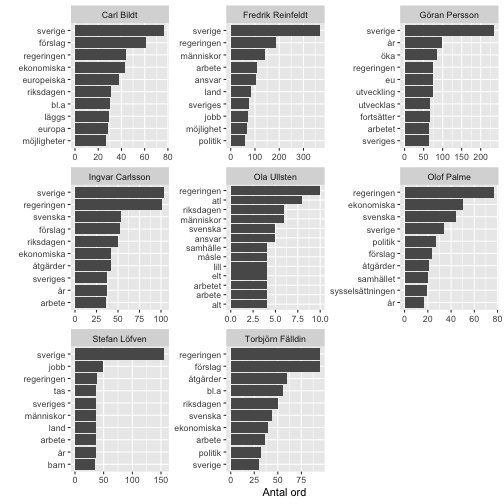
\includegraphics{sl_svd_files/figure-latex/unnamed-chunk-5-1.pdf}

Hur har längden på regeringsförklaringar utvecklats över tid?

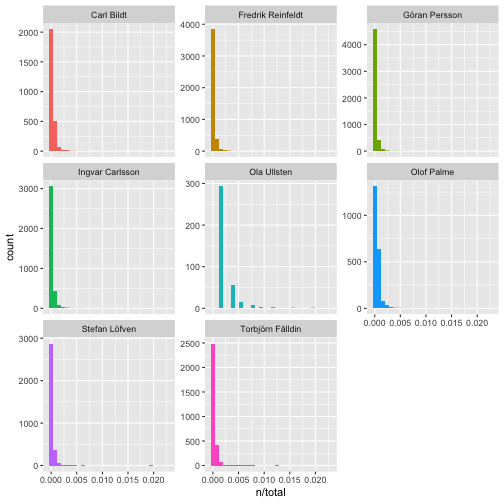
\includegraphics{sl_svd_files/figure-latex/unnamed-chunk-6-1.pdf}

Och hur ser det ut specifikt för Stefan Löfven?

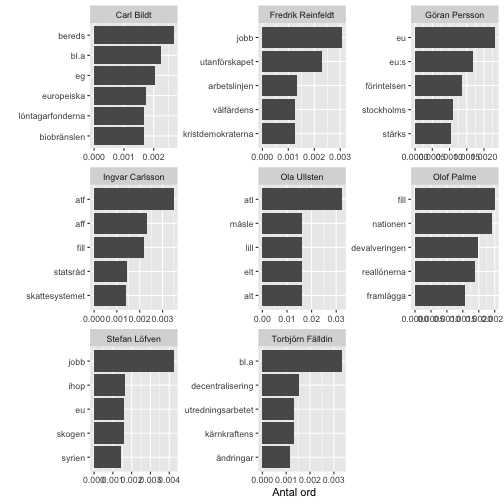
\includegraphics{sl_svd_files/figure-latex/unnamed-chunk-7-1.pdf}

\hypertarget{vilka-ar-stefan-lofvens-viktigaste-ord}{%
\subsection{Vilka är Stefan Löfvens viktigaste
ord?}\label{vilka-ar-stefan-lofvens-viktigaste-ord}}

Att Reinfeldt nämner arbete, ansvar och jobb är inte förvånande och har
ett visst analysvärde, men att Olof Palme nämner regeringen flest gånger
har inget större analytiskt värde, det gör i princip alla andra
statsministrar också.

Det här är ett vanligt problem i analys av text. En metod för att
hantera det här och istället identifiera de \emph{viktigaste} orden i en
text är så kallad \emph{term frequency--inverse document frequency
(tf-idf)}{[}saknar svensk översättning{]}. Principen är, enkelt
uttryckt, att väga upp ord som inte används ofta och väga ner de som
används nästan hela tiden. Metoden utvecklades av matematikern Karen
Spärck Jones. Resultatet av analysen fångar vilka ord som är
``viktigast'' för Stefan Löfvens respektiva regeringsförklaringar.

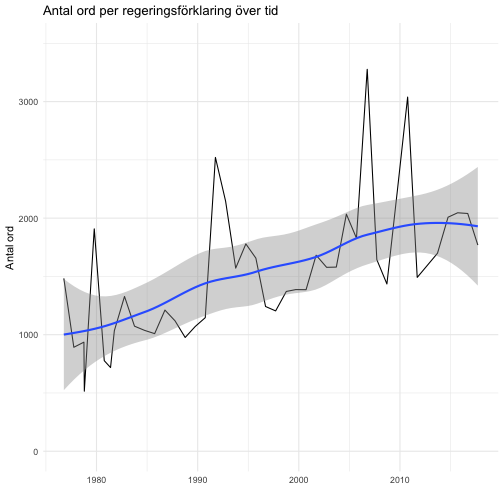
\includegraphics{sl_svd_files/figure-latex/unnamed-chunk-8-1.pdf}

Det sista vi är intresserade av är hur olika ord hänger samman i Stefan
Löfvens regeringsförklaringar. Nedan redovisas relationen mellan ord i
Löfvens regeringsförklaringar.

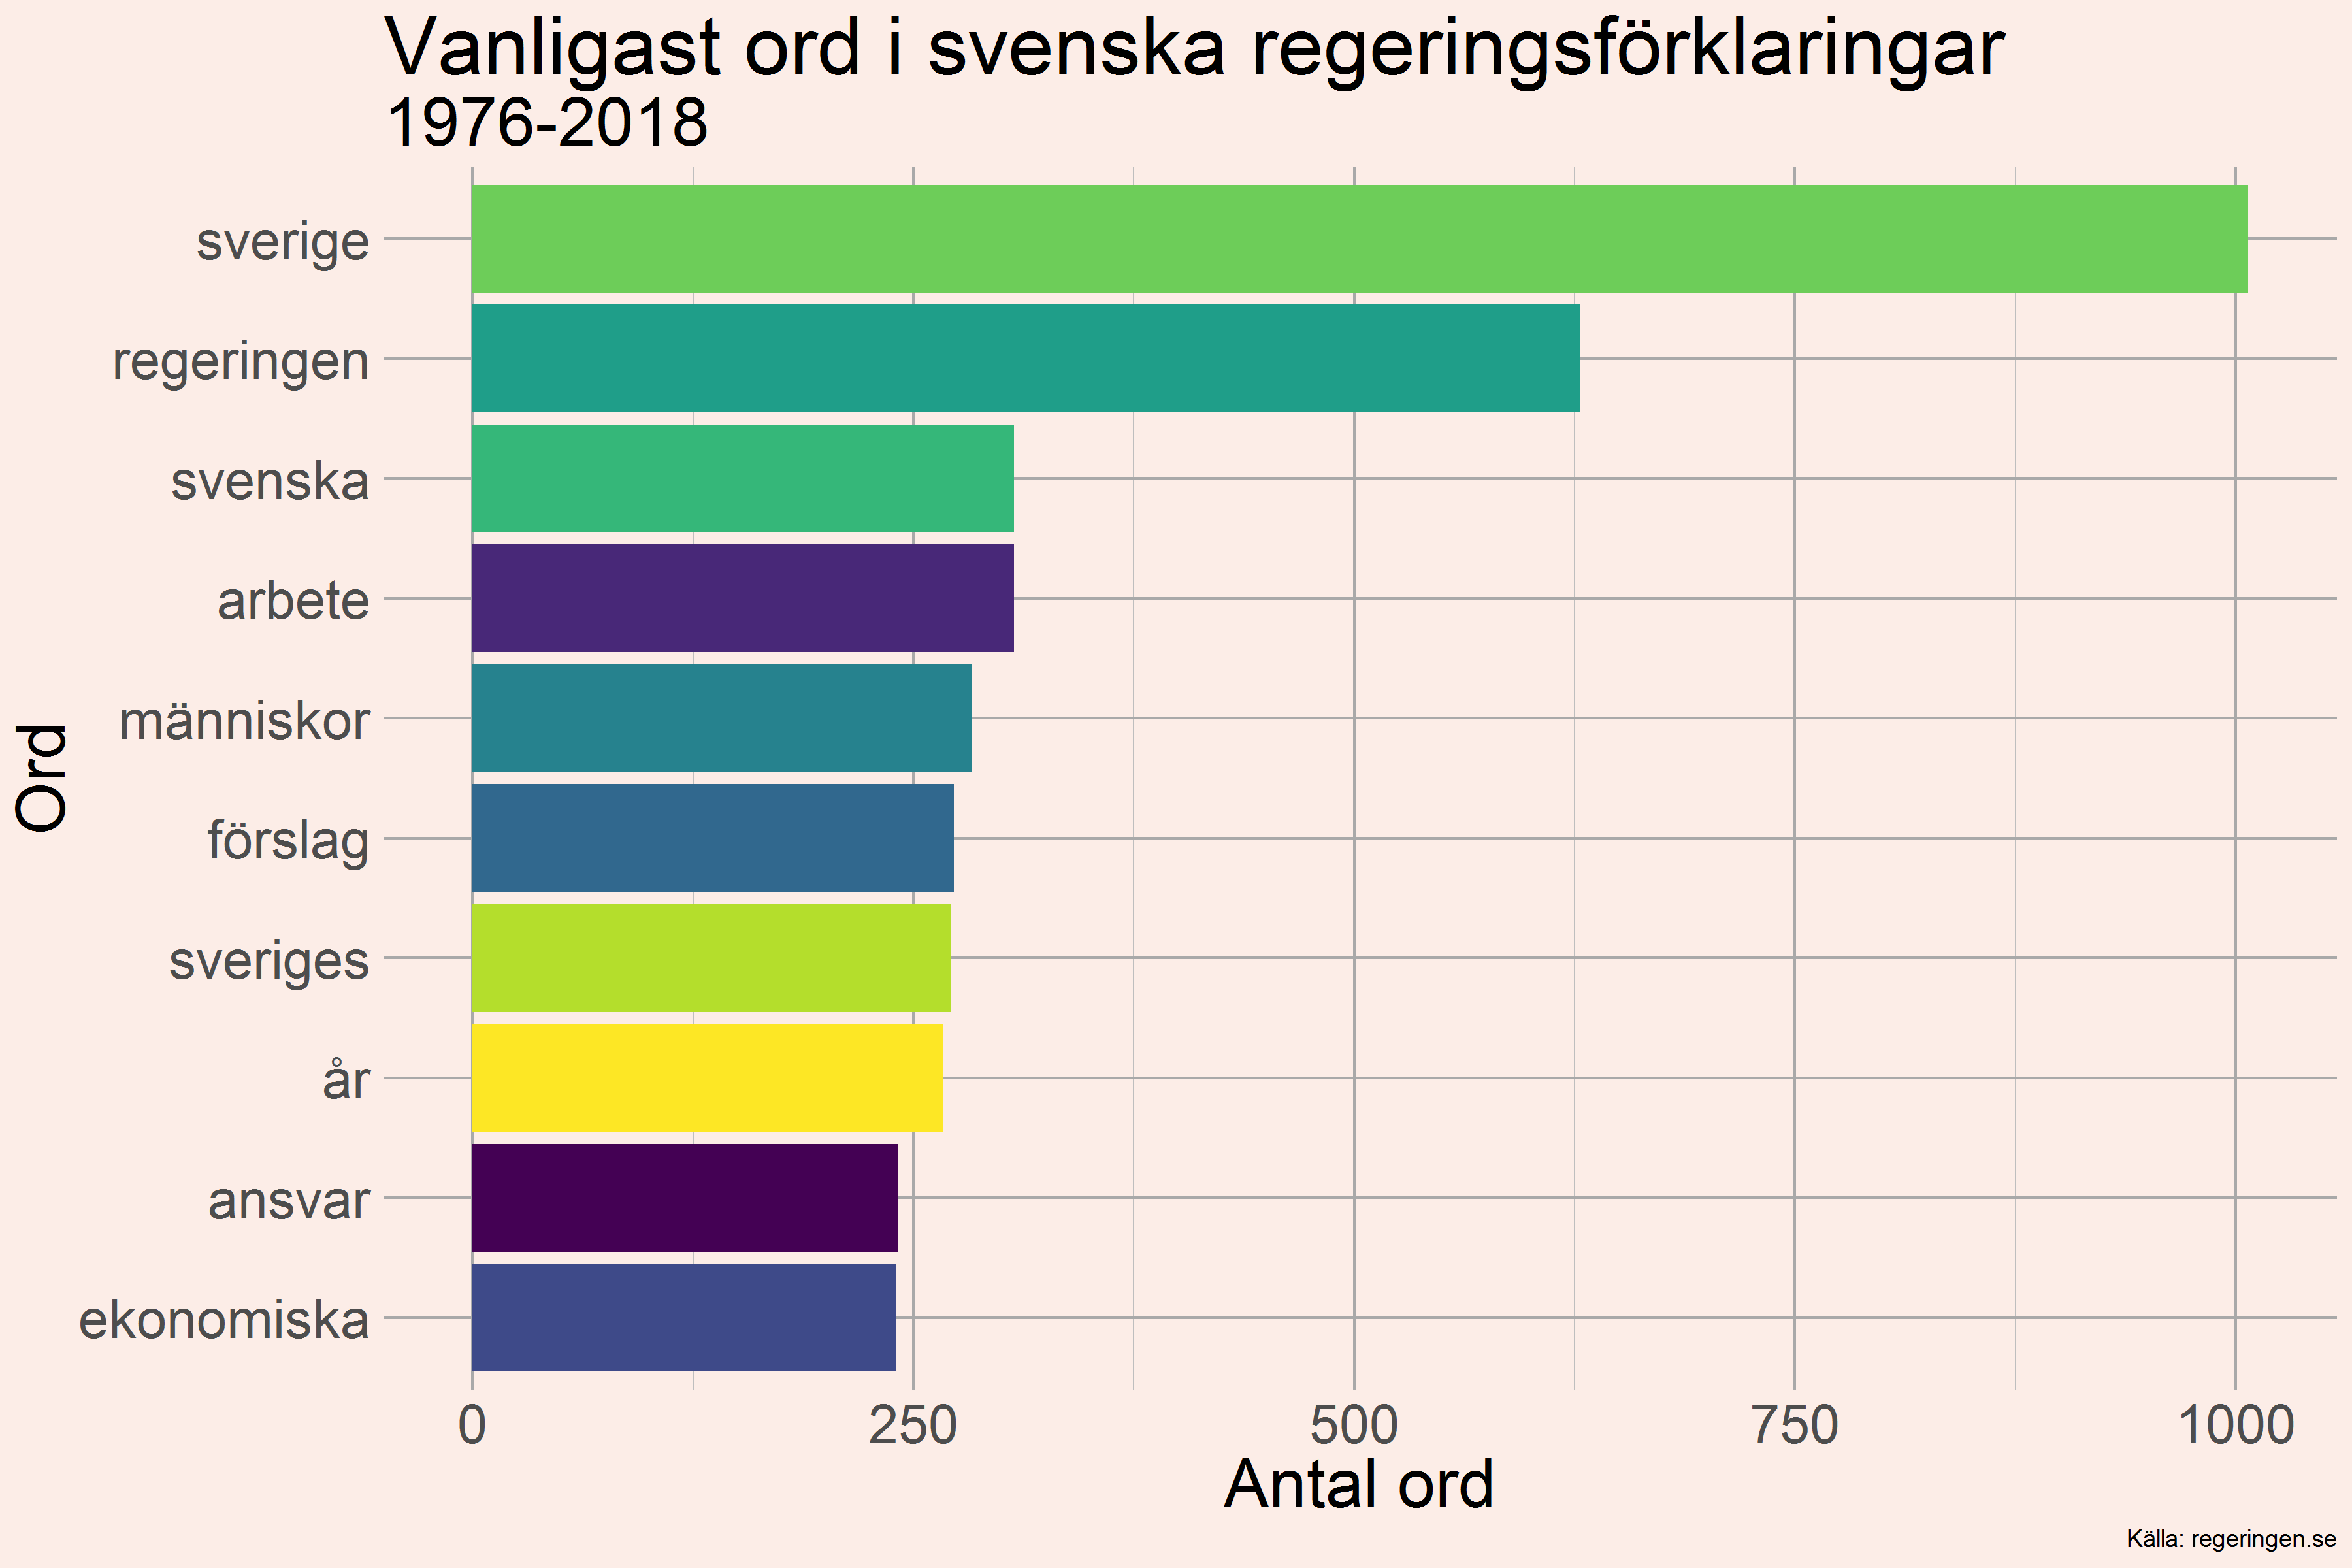
\includegraphics{sl_svd_files/figure-latex/unnamed-chunk-9-1.pdf}


\end{document}
